\documentclass{beamer}
\mode<presentation>
{
  \usetheme{ldv}
  \setbeamercovered{transparent}
}

\usepackage{tikz}
\usetikzlibrary{positioning, arrows.meta}
\newcommand{\slidenomenclature}{Slide}


\usepackage[utf8]{inputenc}
\usepackage{amsmath,amssymb,amsfonts}
\usepackage{times}
\usepackage{graphicx}
\usepackage{fancyvrb}
\usepackage{array}
\usepackage{colortbl}
\usepackage{tabularx}
\usepackage{caption}
\usepackage{adjustbox}

% Preamble
\captionsetup{font=tiny}
\setlength{\parskip}{0pt}
\setbeamertemplate{section in toc}[sections numbered]
\setlength{\parskip}{0pt}
\addtobeamertemplate{section in toc}{}{\vspace{-0.3em}}
\setbeamerfont{page number in head/foot}{size=\small}
\setbeamertemplate{footline}[frame number]

% Header
\newcommand{\zwischentitel}{Cerebellar-Inspired Neural Architectures}
\newcommand{\leitthema}{Guilherme Simões}
% End Header

% Titlepage
\title{Cerebellar-Inspired Neural Architectures for Motor Learning in Simulated Environments}

\author{Guilherme Simões}
\newcommand{\presdatum}{August 2026}
\institute
{
  NOVA FCT\\
}

\begin{document}
  \begin{frame}
    \titlepage
  \end{frame}

  \begin{frame}
    \frametitle{Outline}
    \small
    \tableofcontents[sections={1-20},hideallsubsections]
  \end{frame}


  \section{Motivation}
    \begin{frame}
      \frametitle{Motivation}
      \begin{block}<1->{The Challenge}
          Learning motor skills requires coordinating movements over
          time, adapting to different goals and correcting errors
          based on feedback.
      \end{block}

      \vspace{0.3cm}

      \begin{columns}[T]
          \begin{column}{0.48\textwidth}
              \begin{block}<2->{Supervised Learning}
                  Uses prediction errors to improve movement execution.
              \end{block}
          \end{column}

          \begin{column}{0.48\textwidth}
              \begin{block}<3->{Reinforcement Learning}
                  Uses reward feedback to improve action selection.
              \end{block}
          \end{column}
      \end{columns}

      \vspace{0.3cm}

      \begin{block}<4->{Research Question}
          Can biologically inspired learning mechanisms improve
          the efficiency, reliability and generalization of
          motor learning?
      \end{block}
  \end{frame}

  % Explicar que o objetivo atual é tentar combinar ambas a SL e RL approaches para criar uma arquitetura híbrida funcional

  \section{Introduction}
    \begin{frame}
      \frametitle{Introduction}
        \hspace{0.3cm} This thesis will be based on two papers:
        \vspace{0.5cm}
        \begin{itemize}
          \item Cerebellar-driven cortical dynamics can enable task acquisition, switching and consolidation $\rightarrow$ SL approach
          \vspace{0.3cm}
          \item Policy-Gradient Reinforcement Learning as a General Theory of Practice-Based Motor Skill Learning $\rightarrow$ RL approach
        \end{itemize}
    \end{frame}

  \section{Cerebellar-driven cortical dynamics}
    \begin{frame}
      \frametitle{Cerebellar-driven Cortical Dynamics Approach}
      \begin{figure}
        \centering
        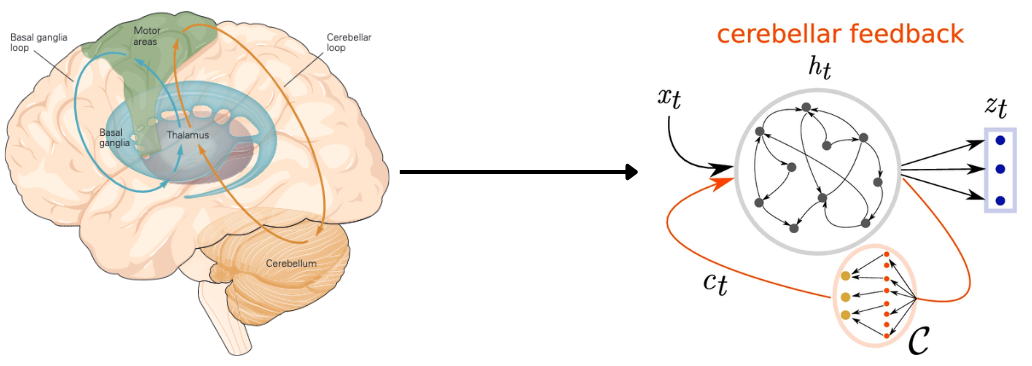
\includegraphics[scale=0.3]{images/cerebellarRepresentation.png}
        \caption{Cerebro-cerebellar network architecture}
      \end{figure}
    \end{frame}

    % a copy of RNN activity (ht) is sent to a (feedforward) cerebellar network C, which feedbacks to the cortical network its own cerebellar predictions (ct).

\begin{frame}
    \frametitle{Modeled Cerebellar Feedback Loop}

    \centering

    \only<1>{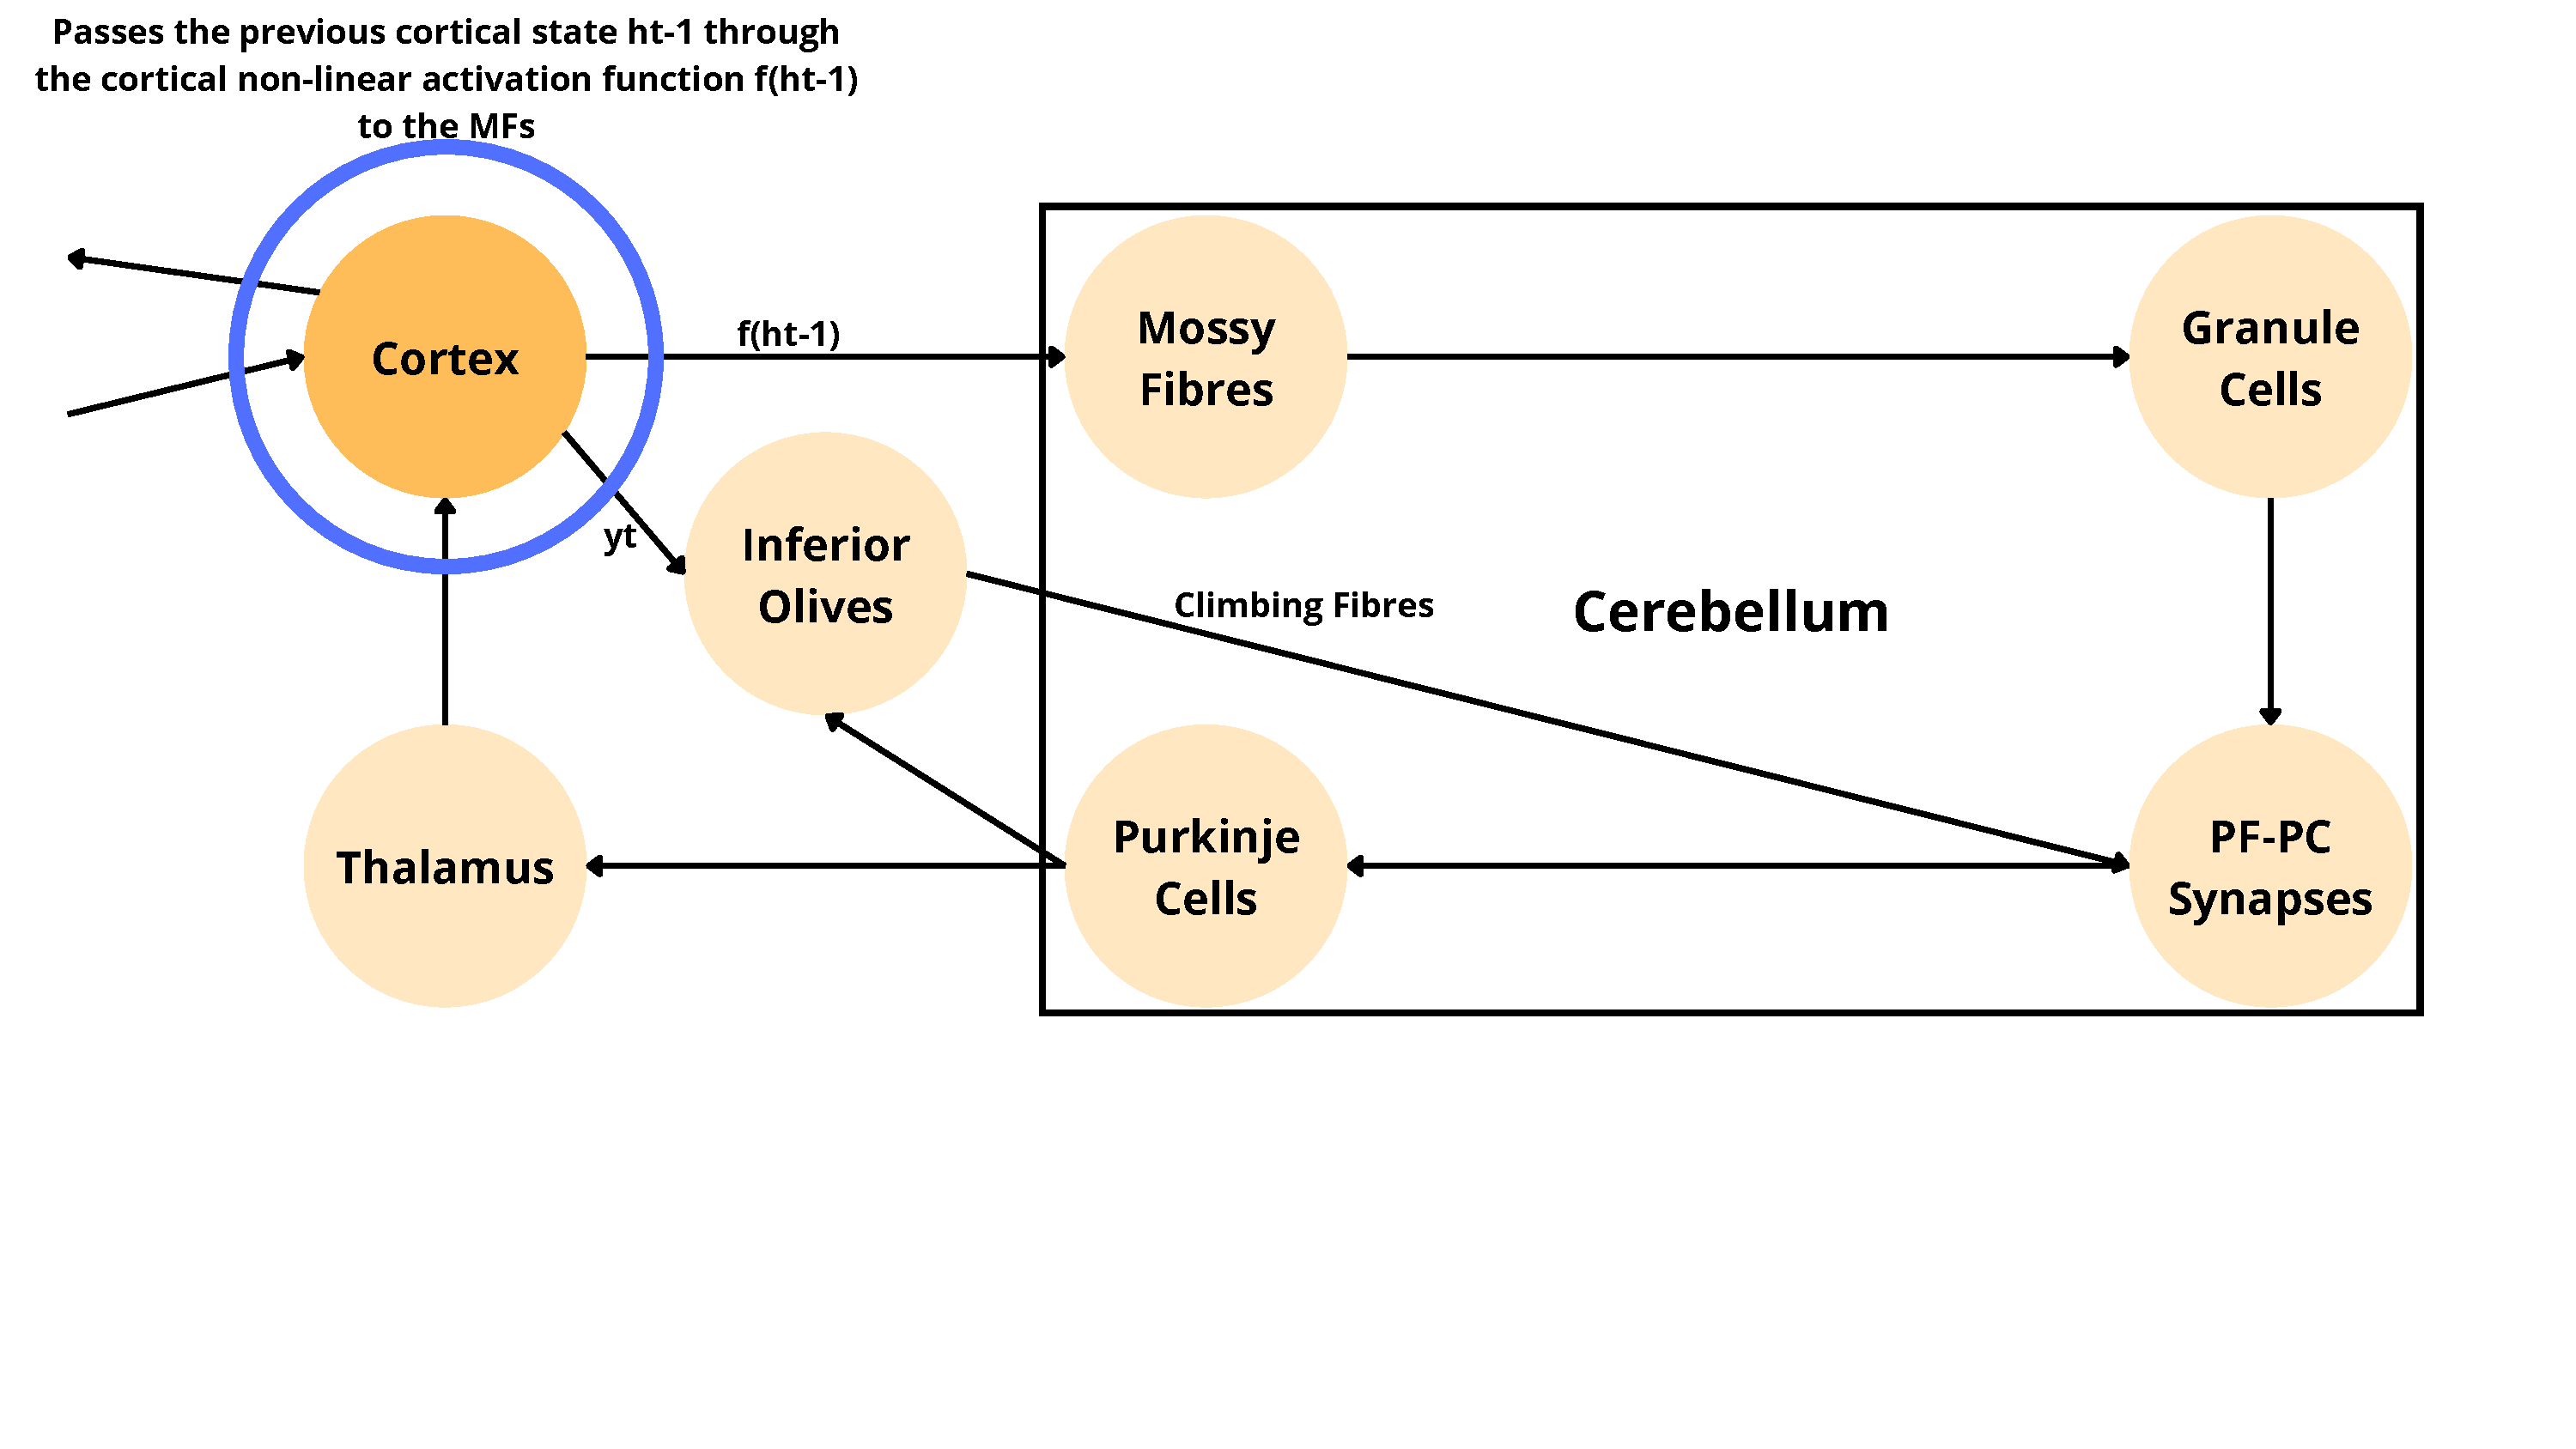
\includegraphics[scale=0.23]{images/cerebellarLoopSchematic/Schema1.pdf}}
    \only<2>{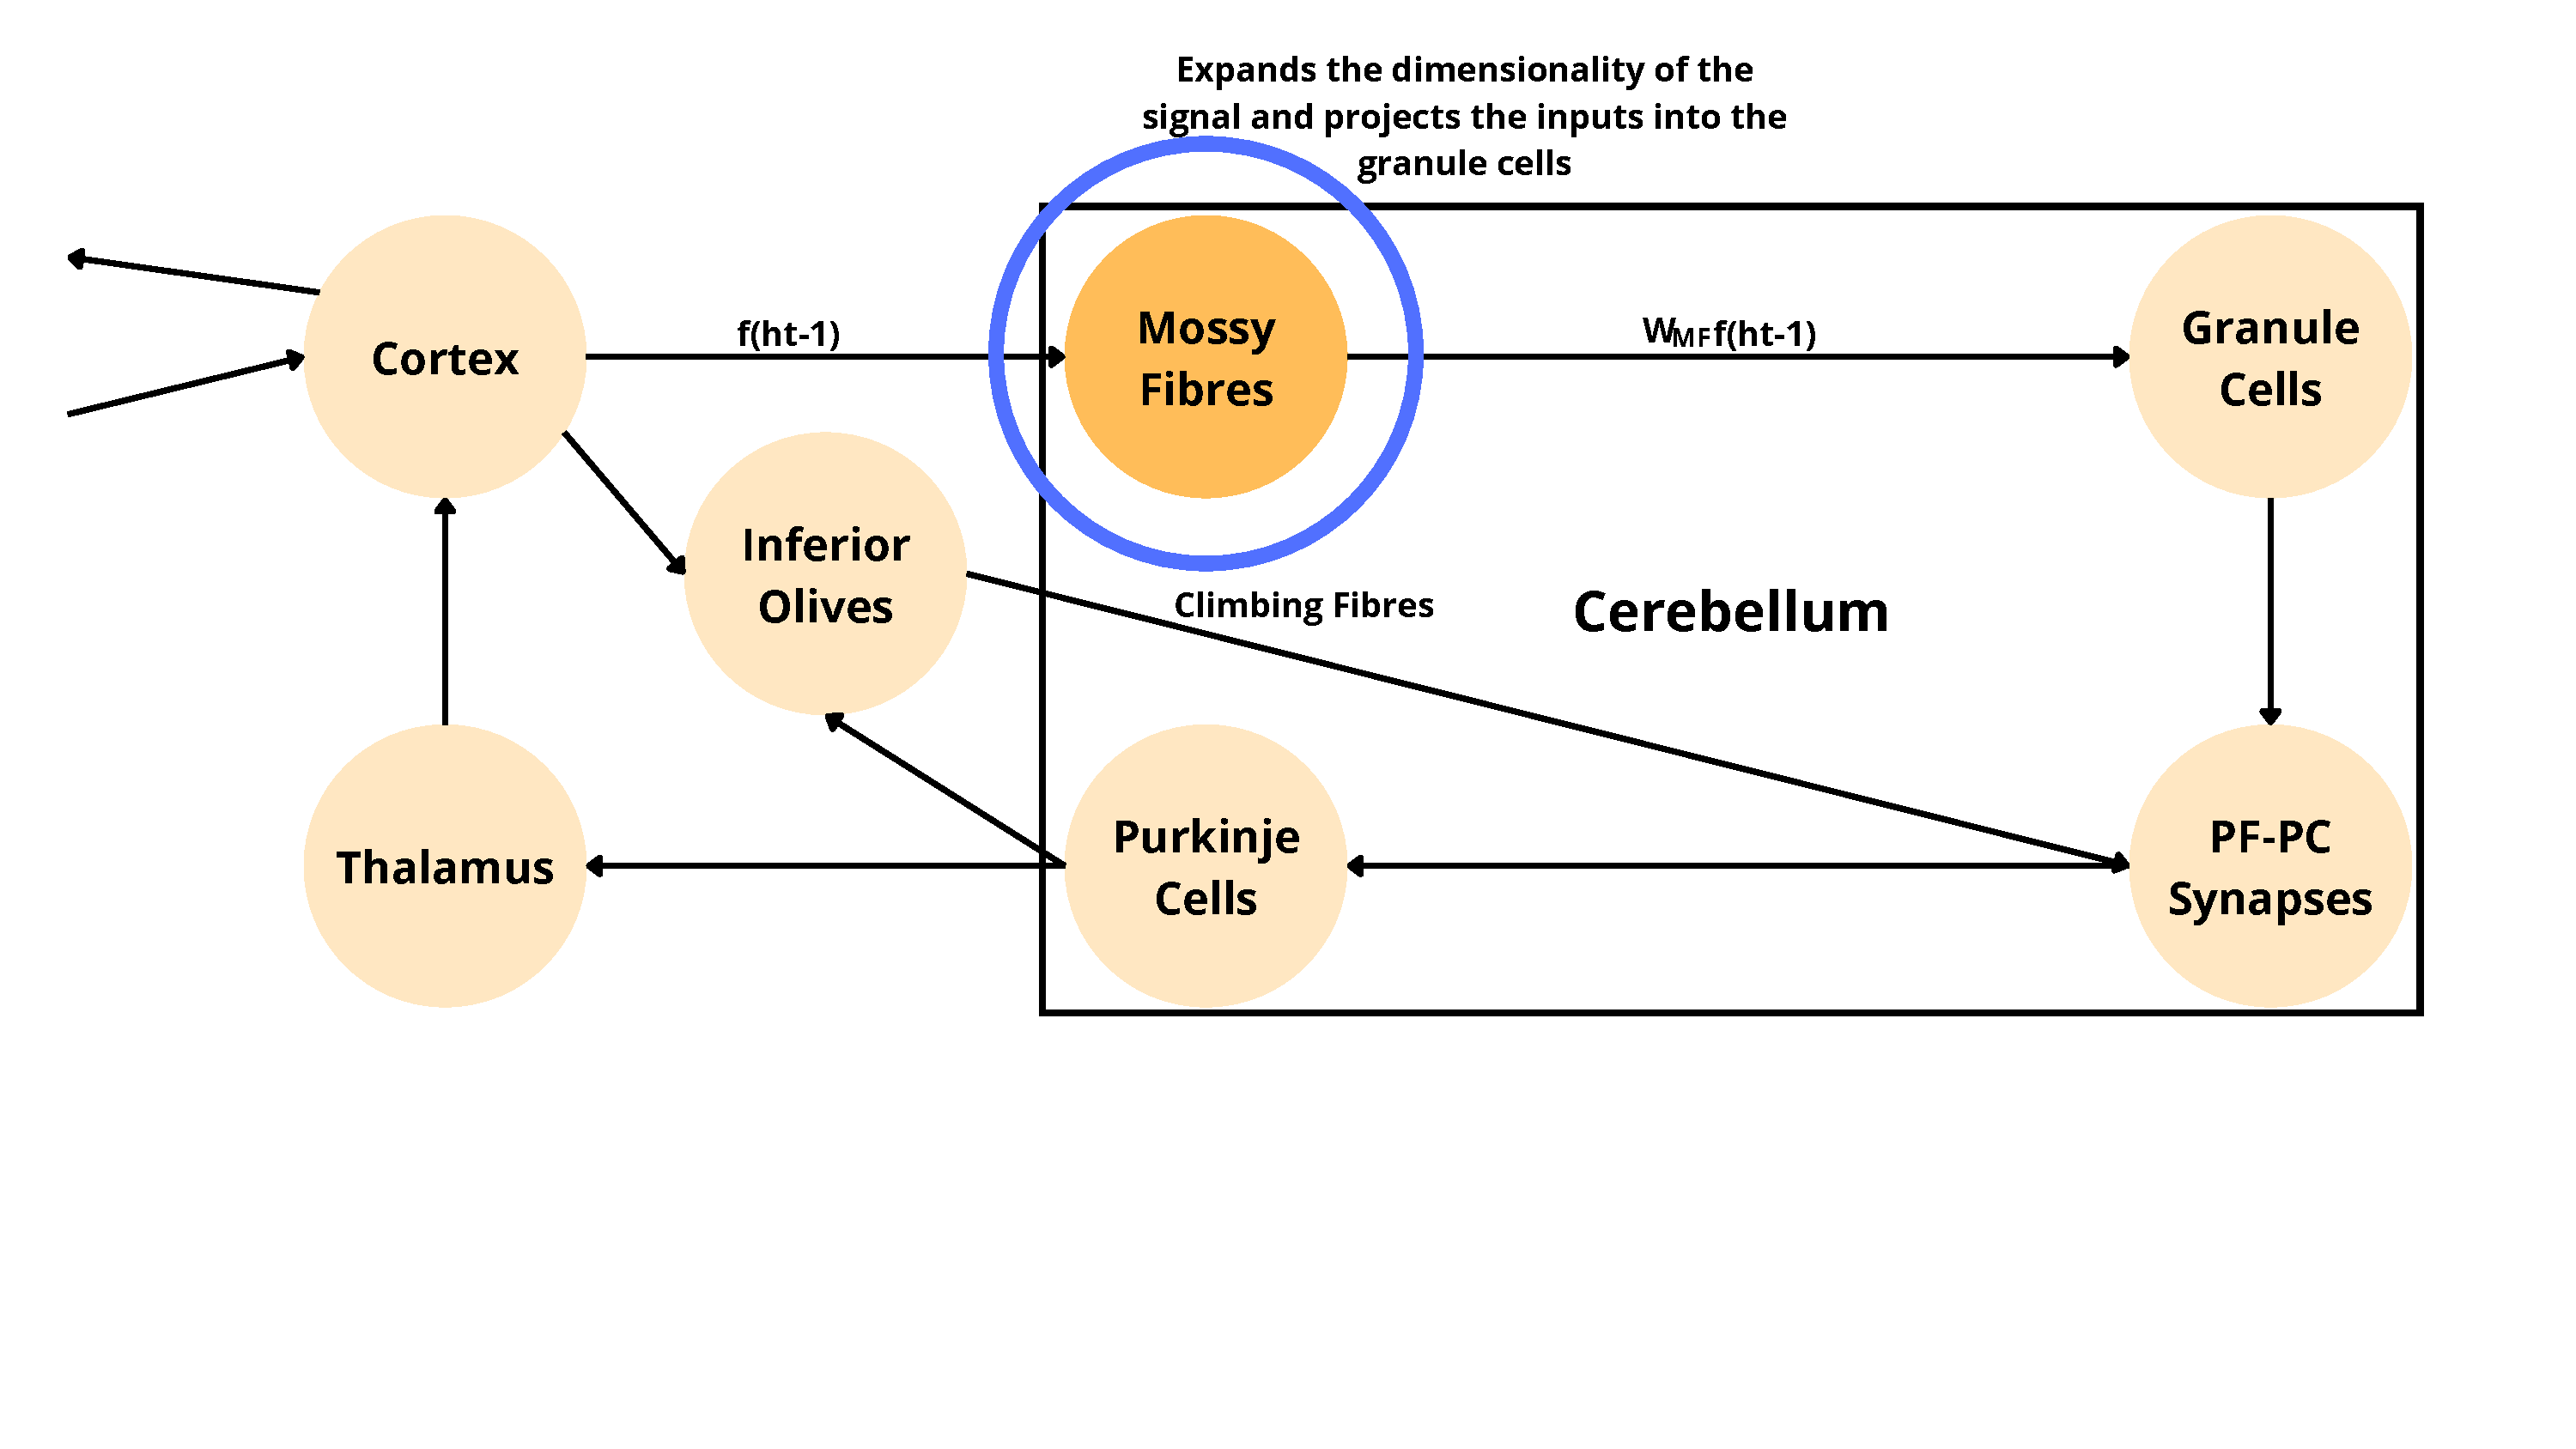
\includegraphics[scale=0.23]{images/cerebellarLoopSchematic/Schema2.pdf}}
    \only<3>{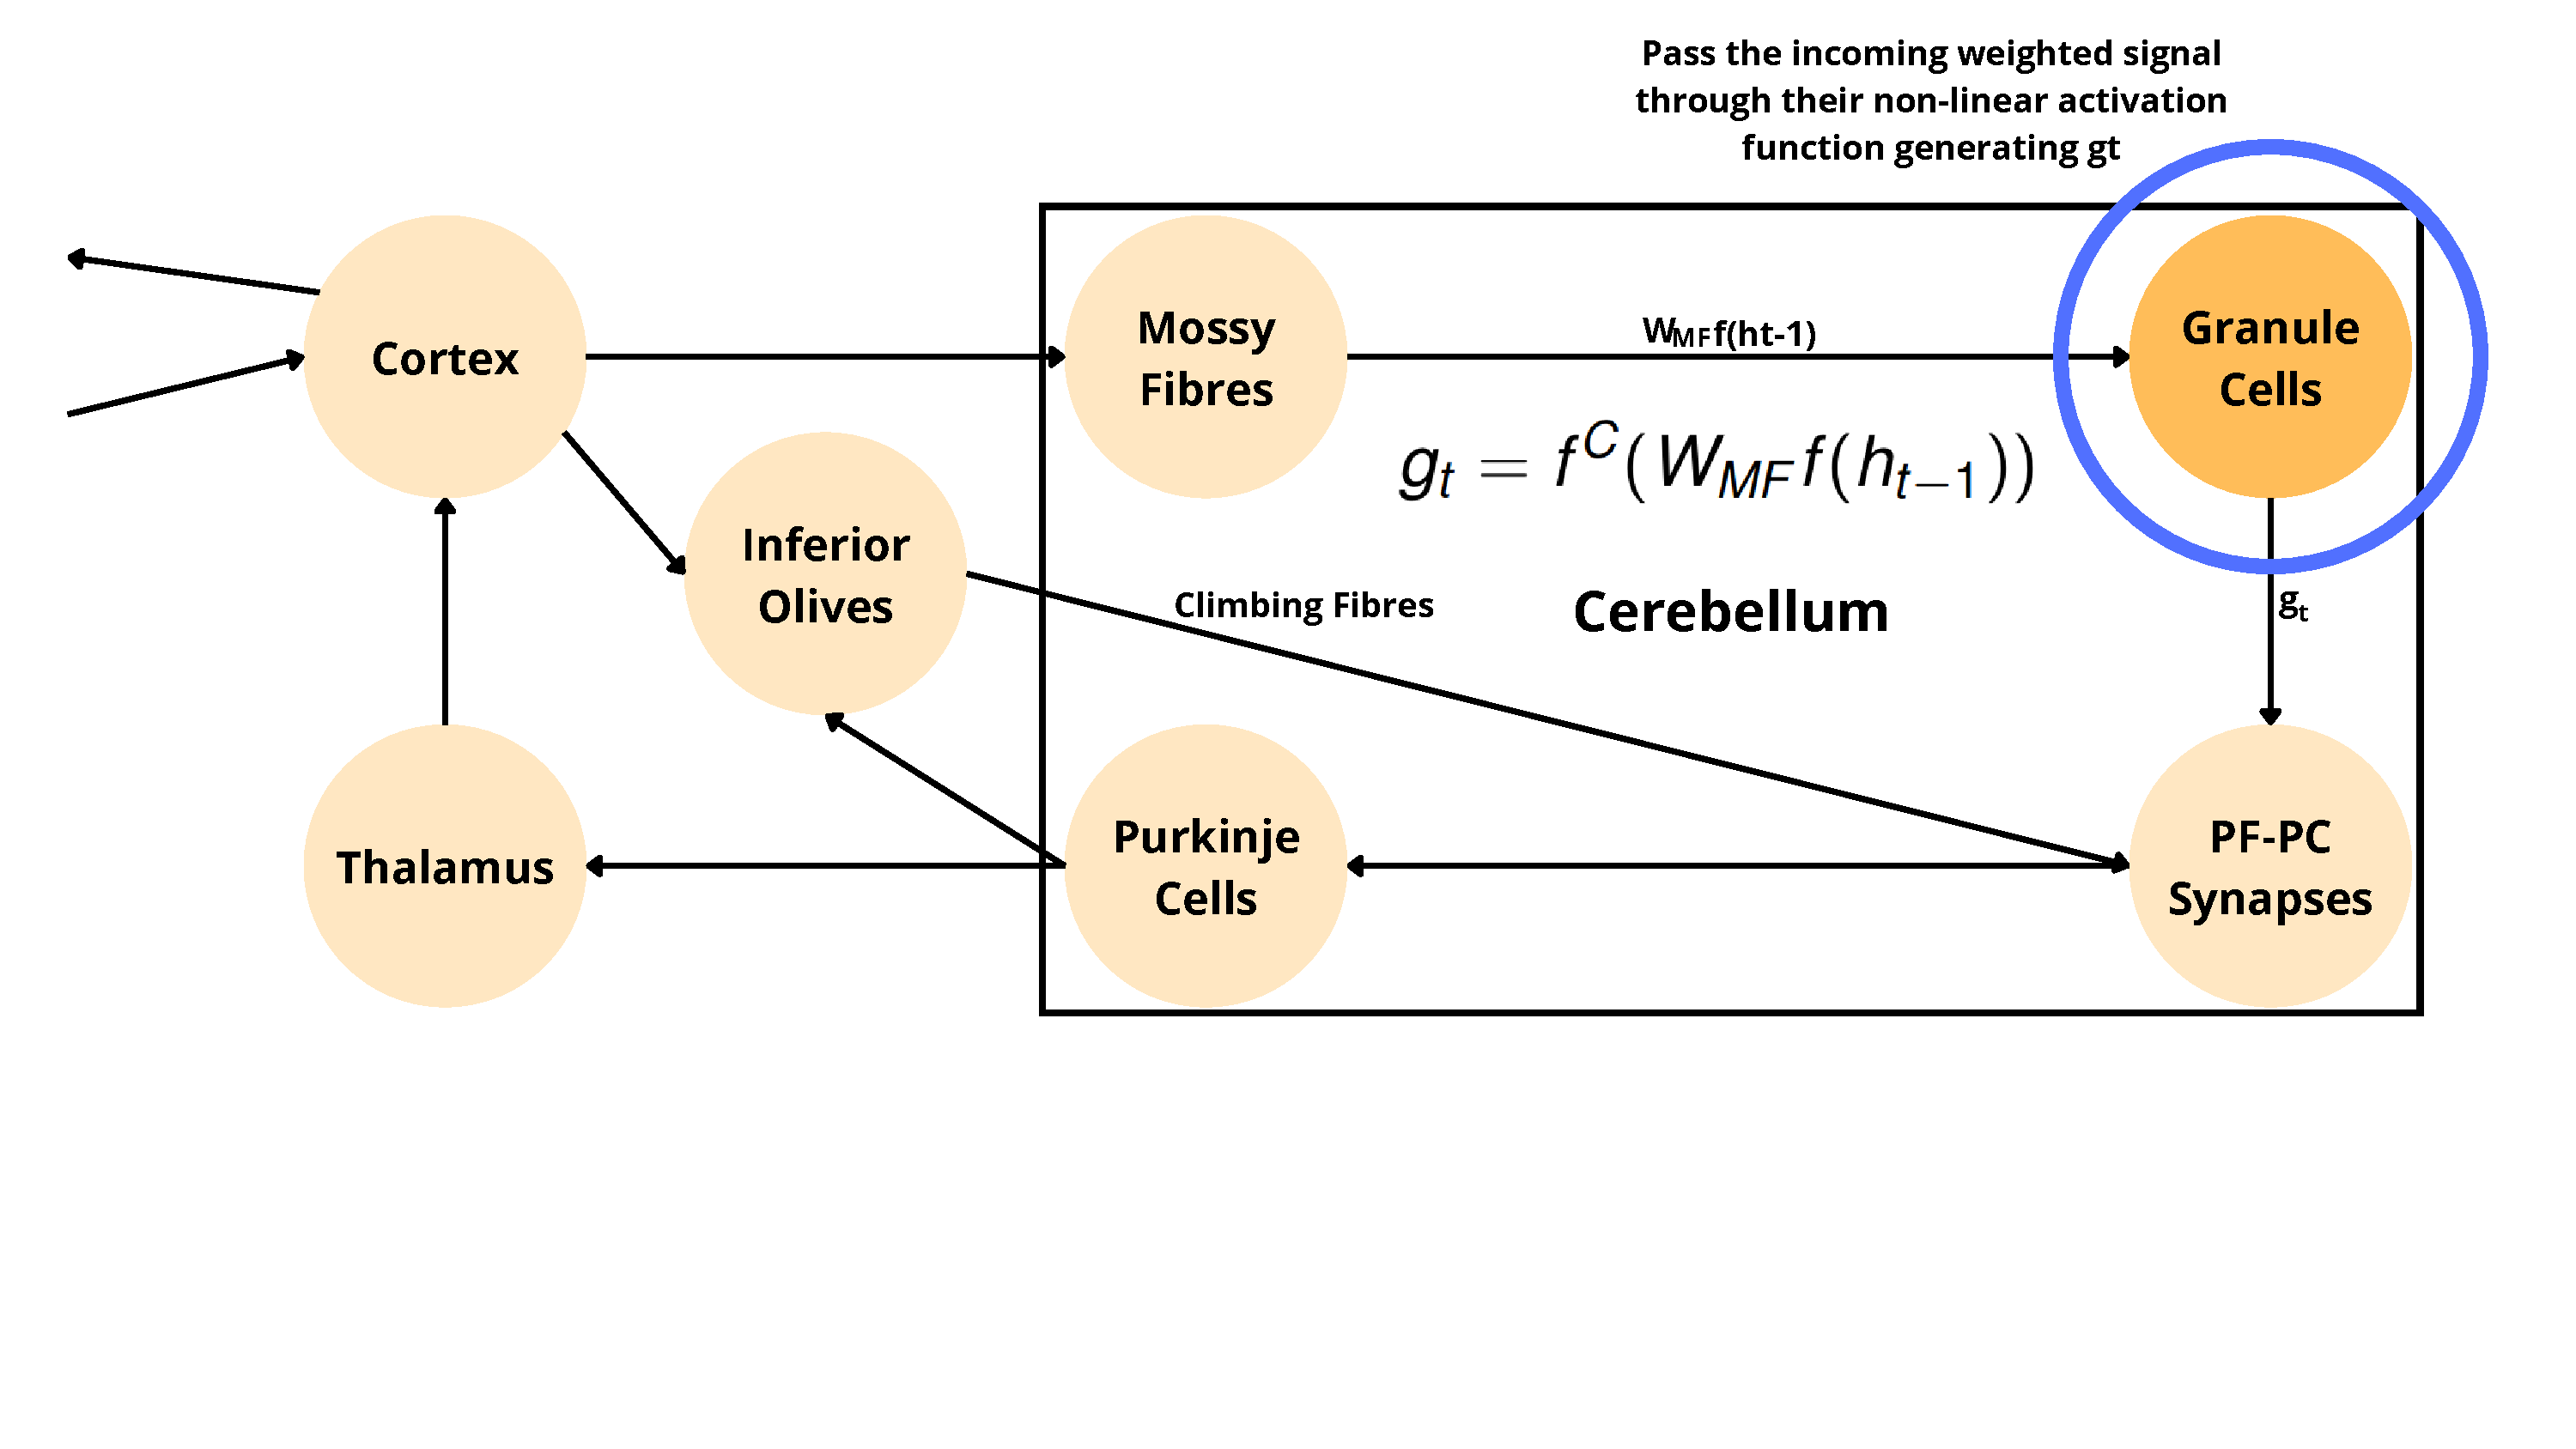
\includegraphics[scale=0.23]{images/cerebellarLoopSchematic/Schema3.pdf}}
    \only<4>{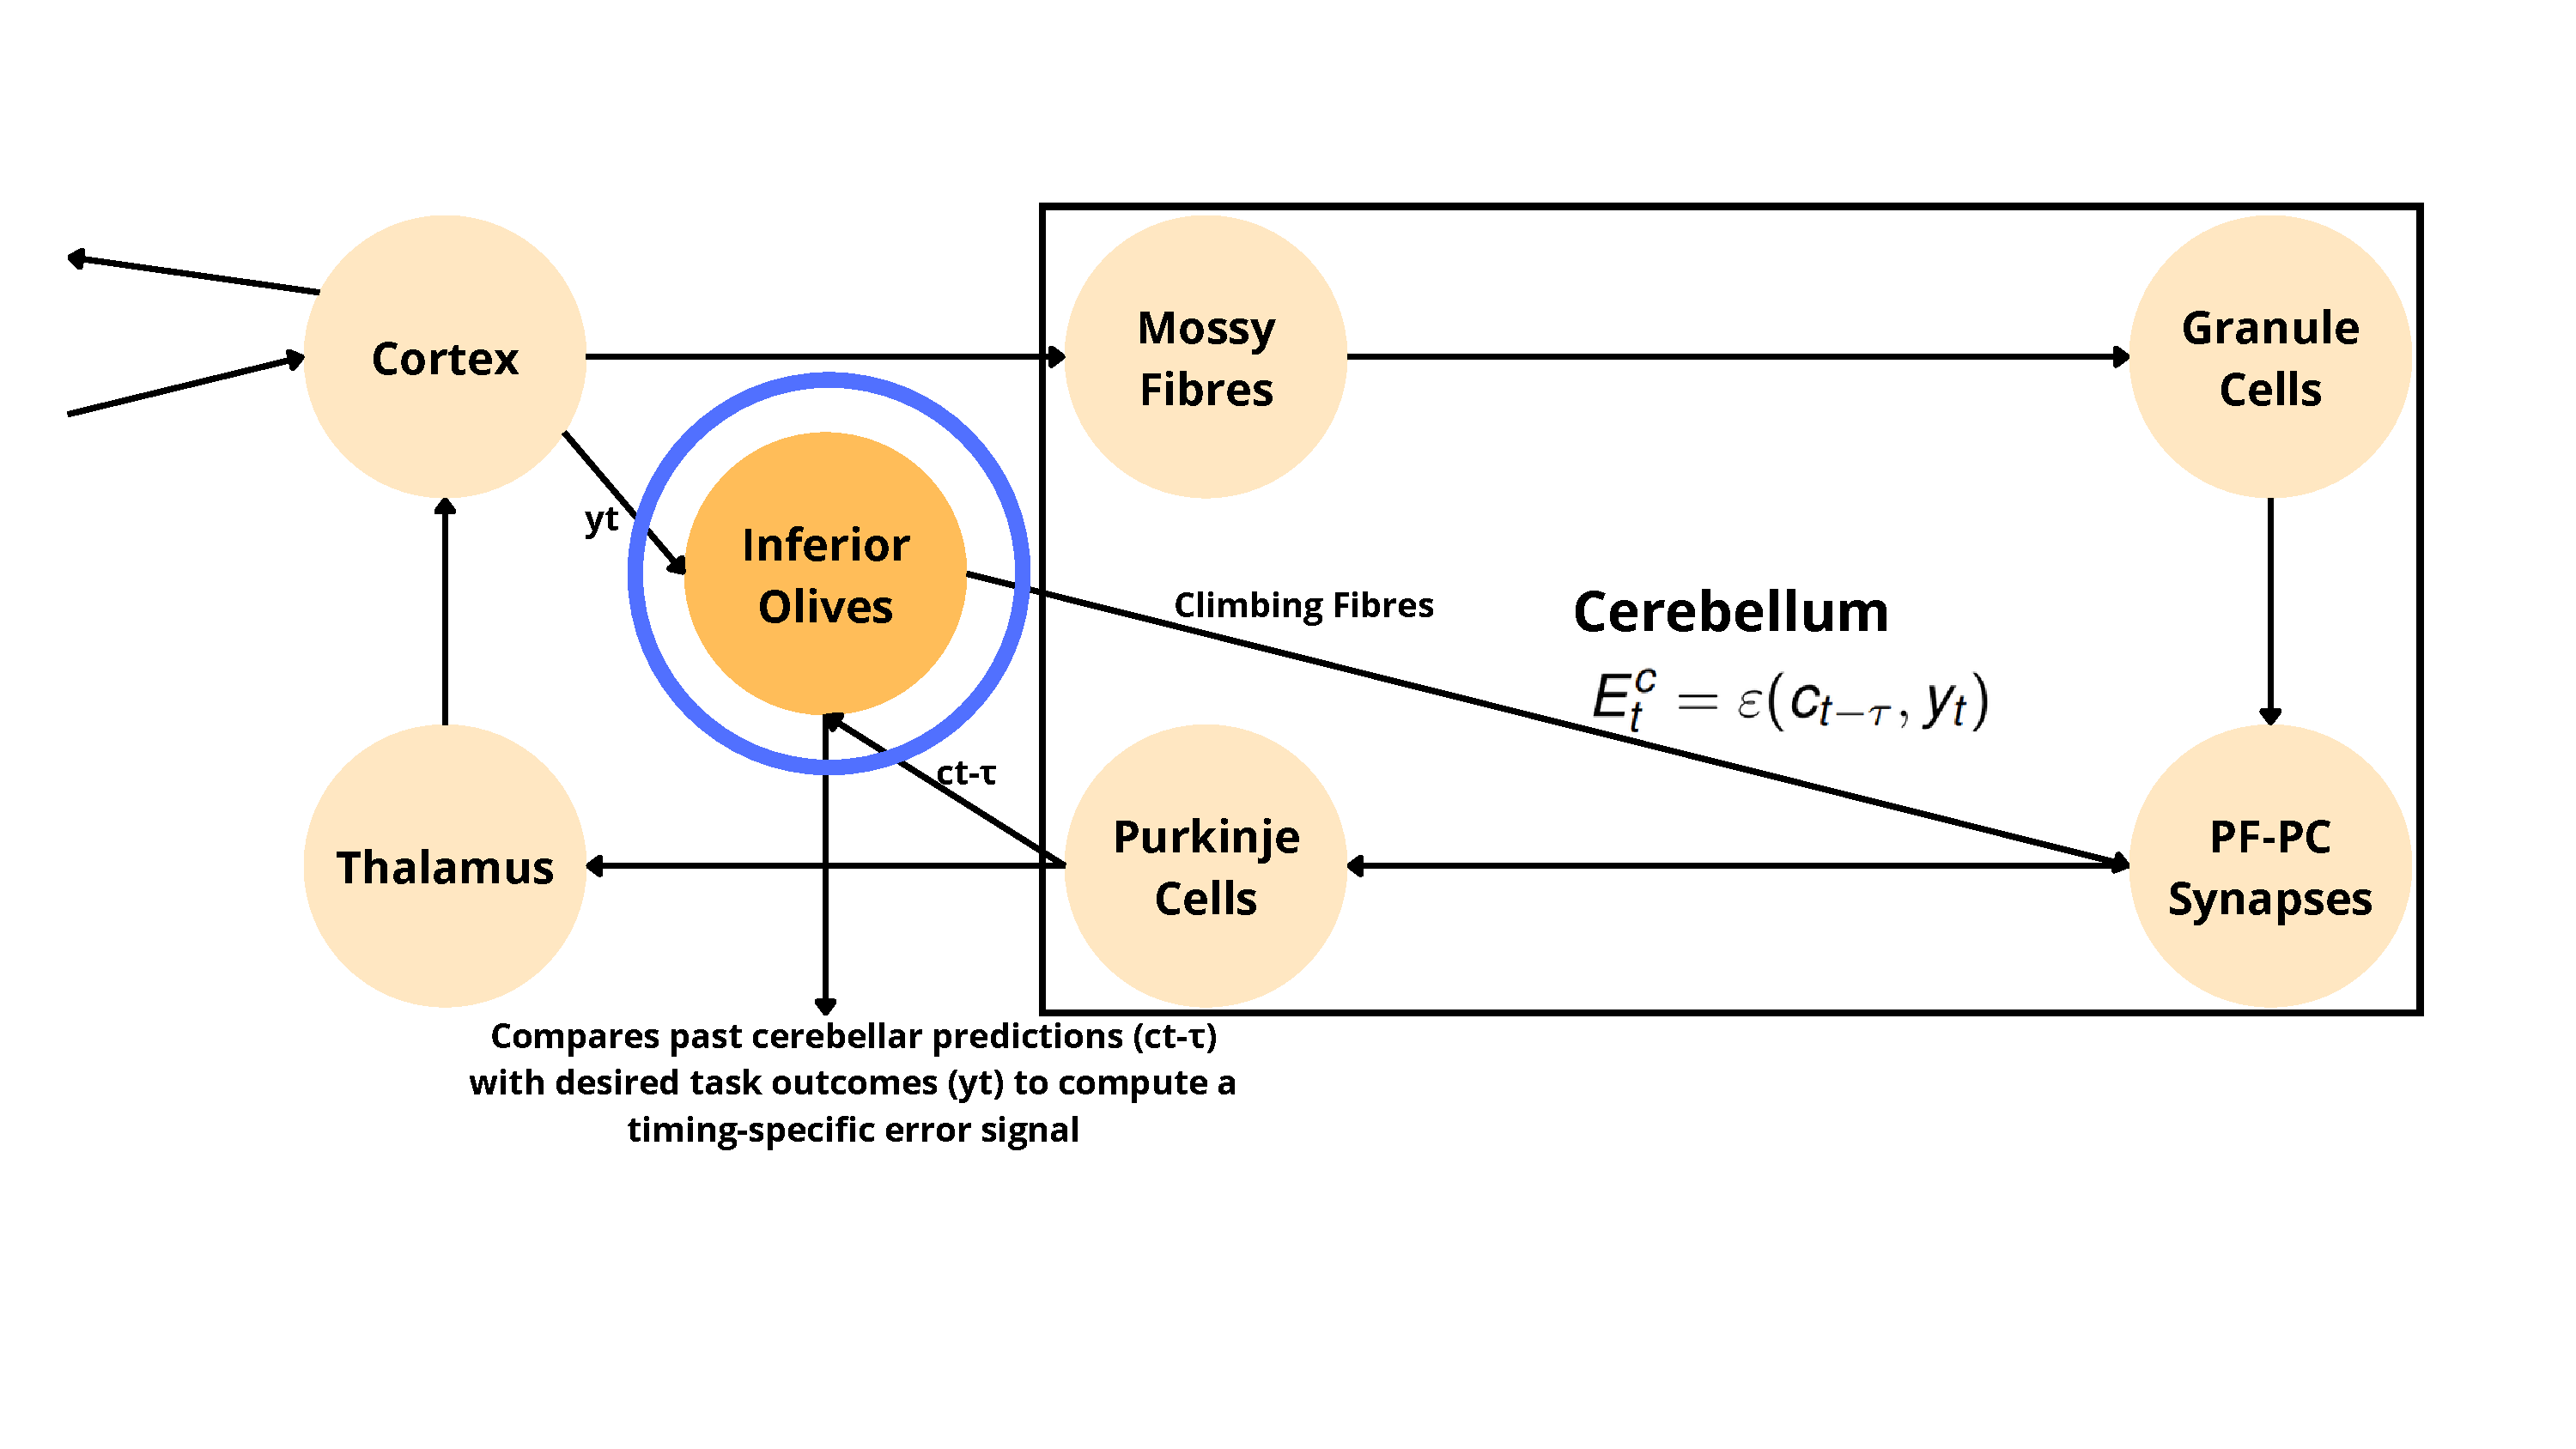
\includegraphics[scale=0.23]{images/cerebellarLoopSchematic/Schema4.pdf}}
    \only<5>{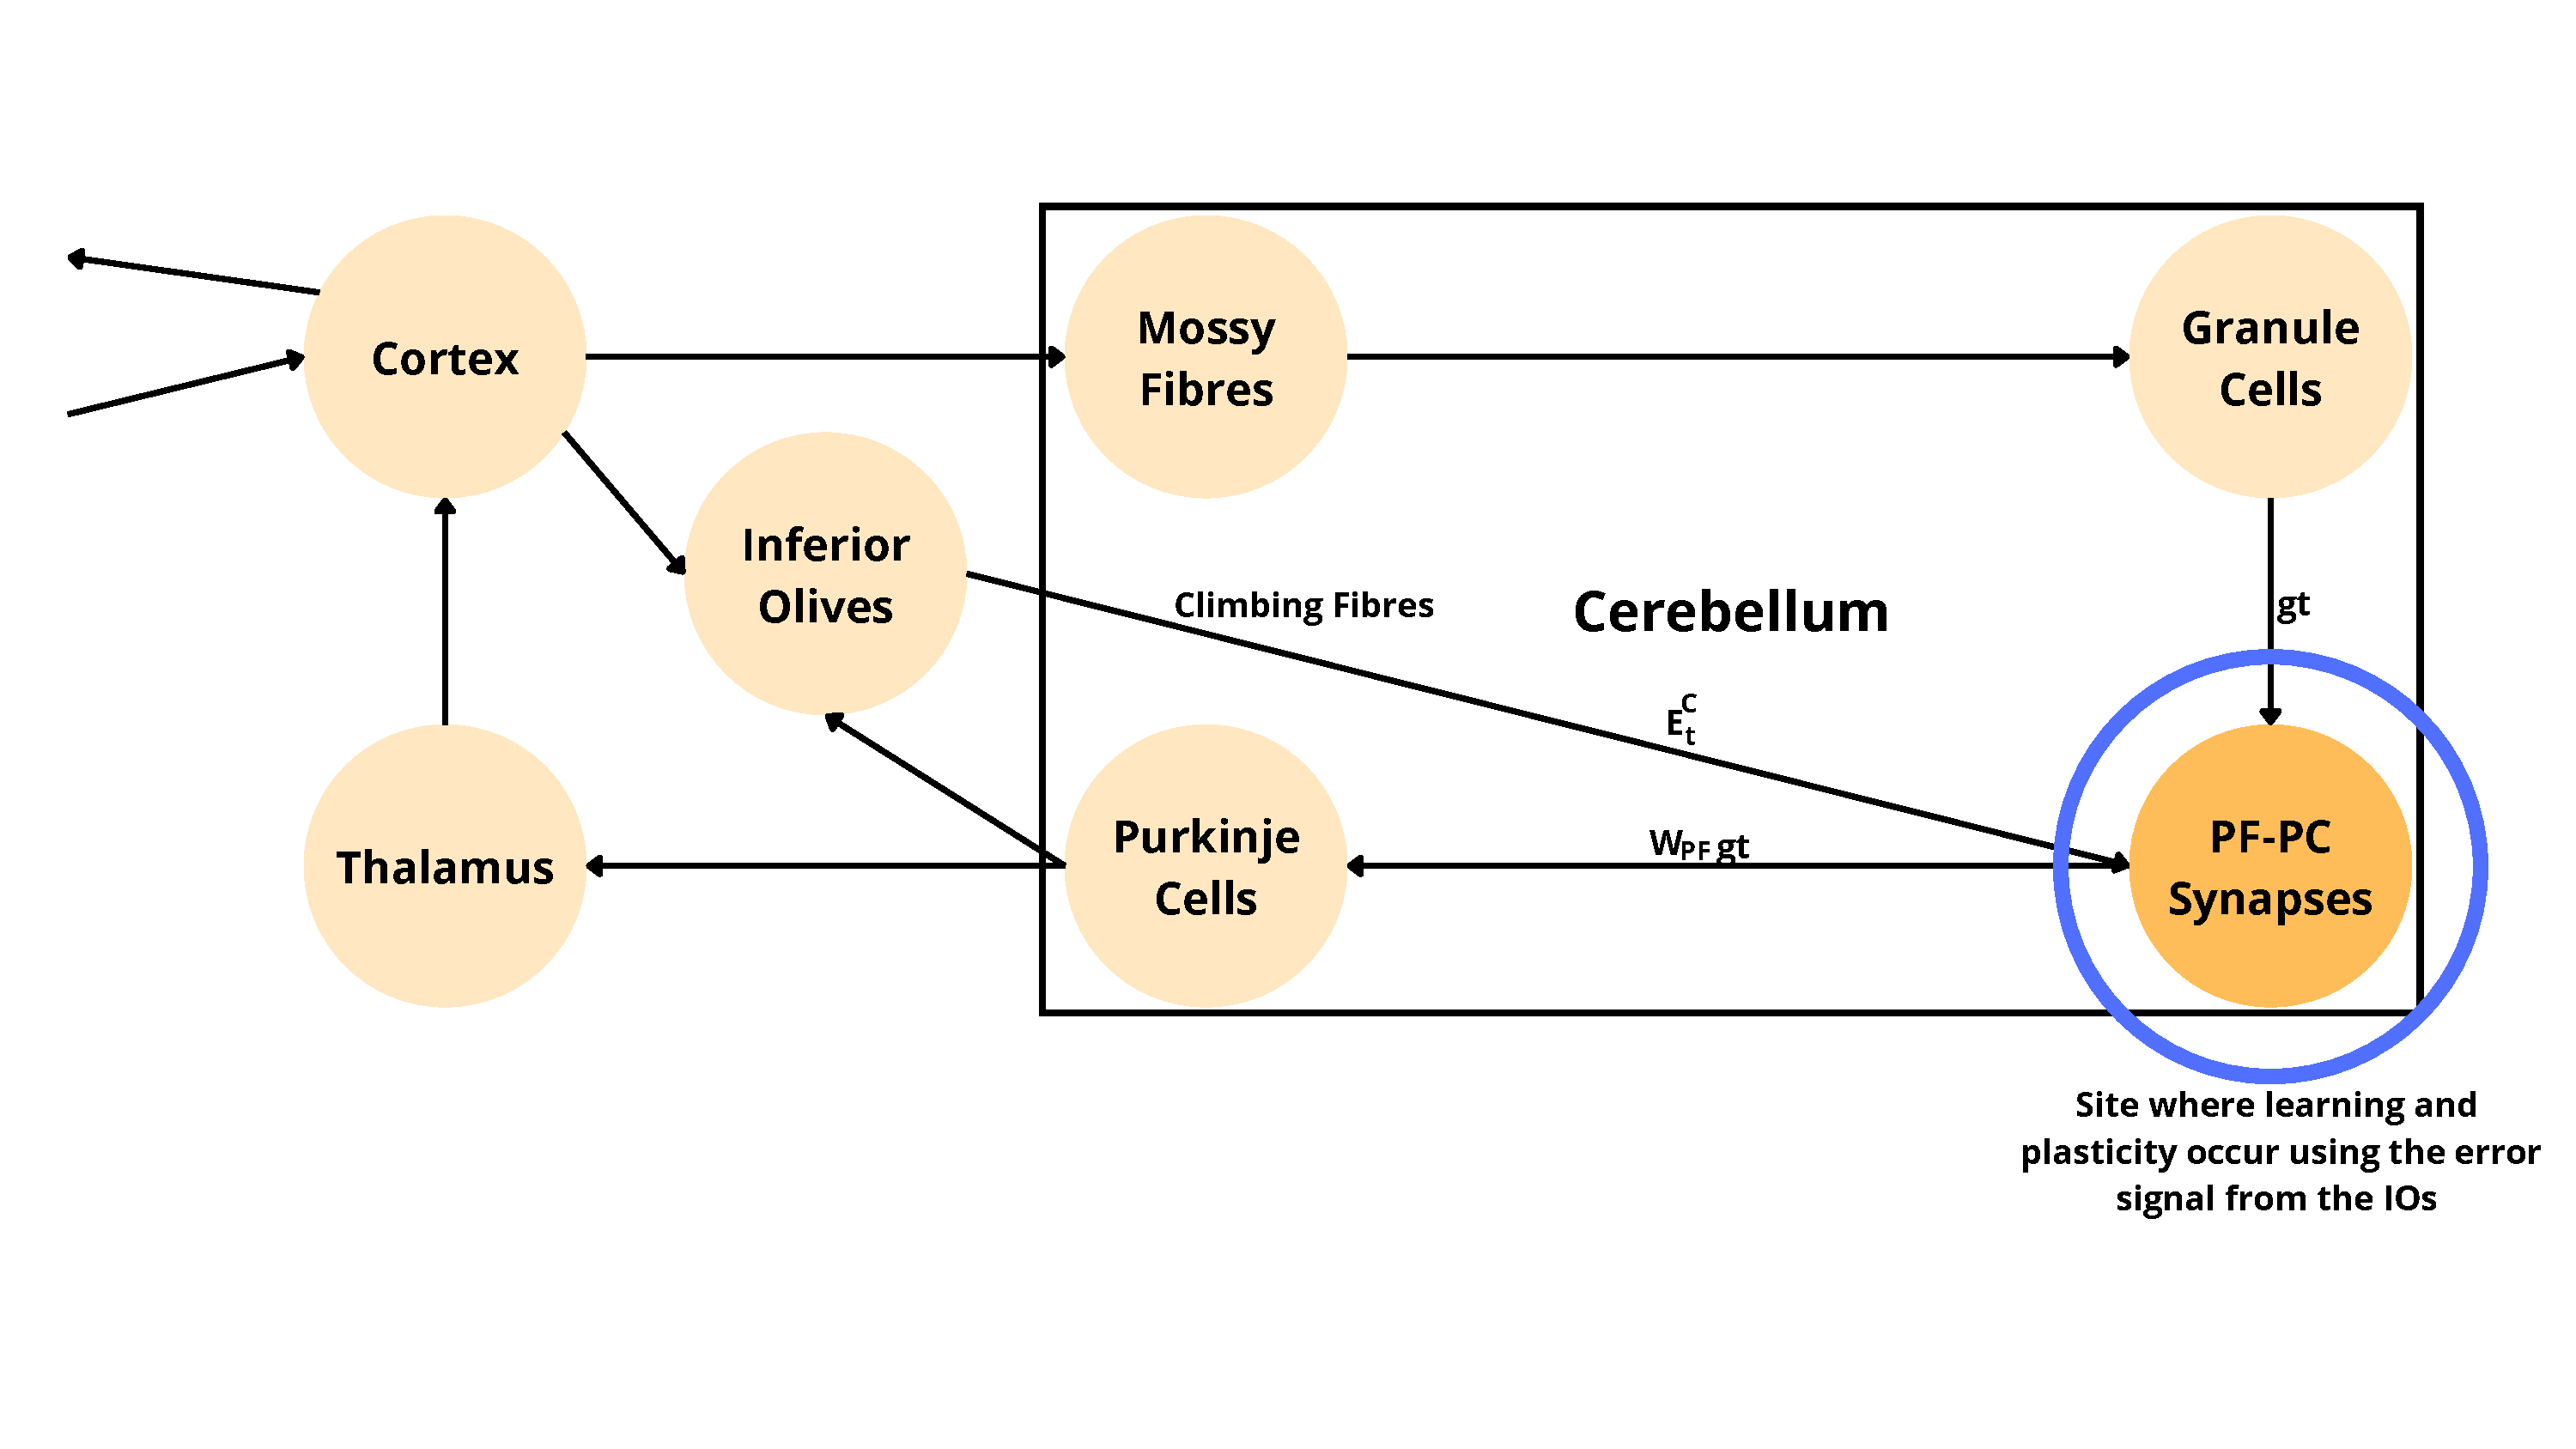
\includegraphics[scale=0.23]{images/cerebellarLoopSchematic/Schema5.pdf}}
    \only<6>{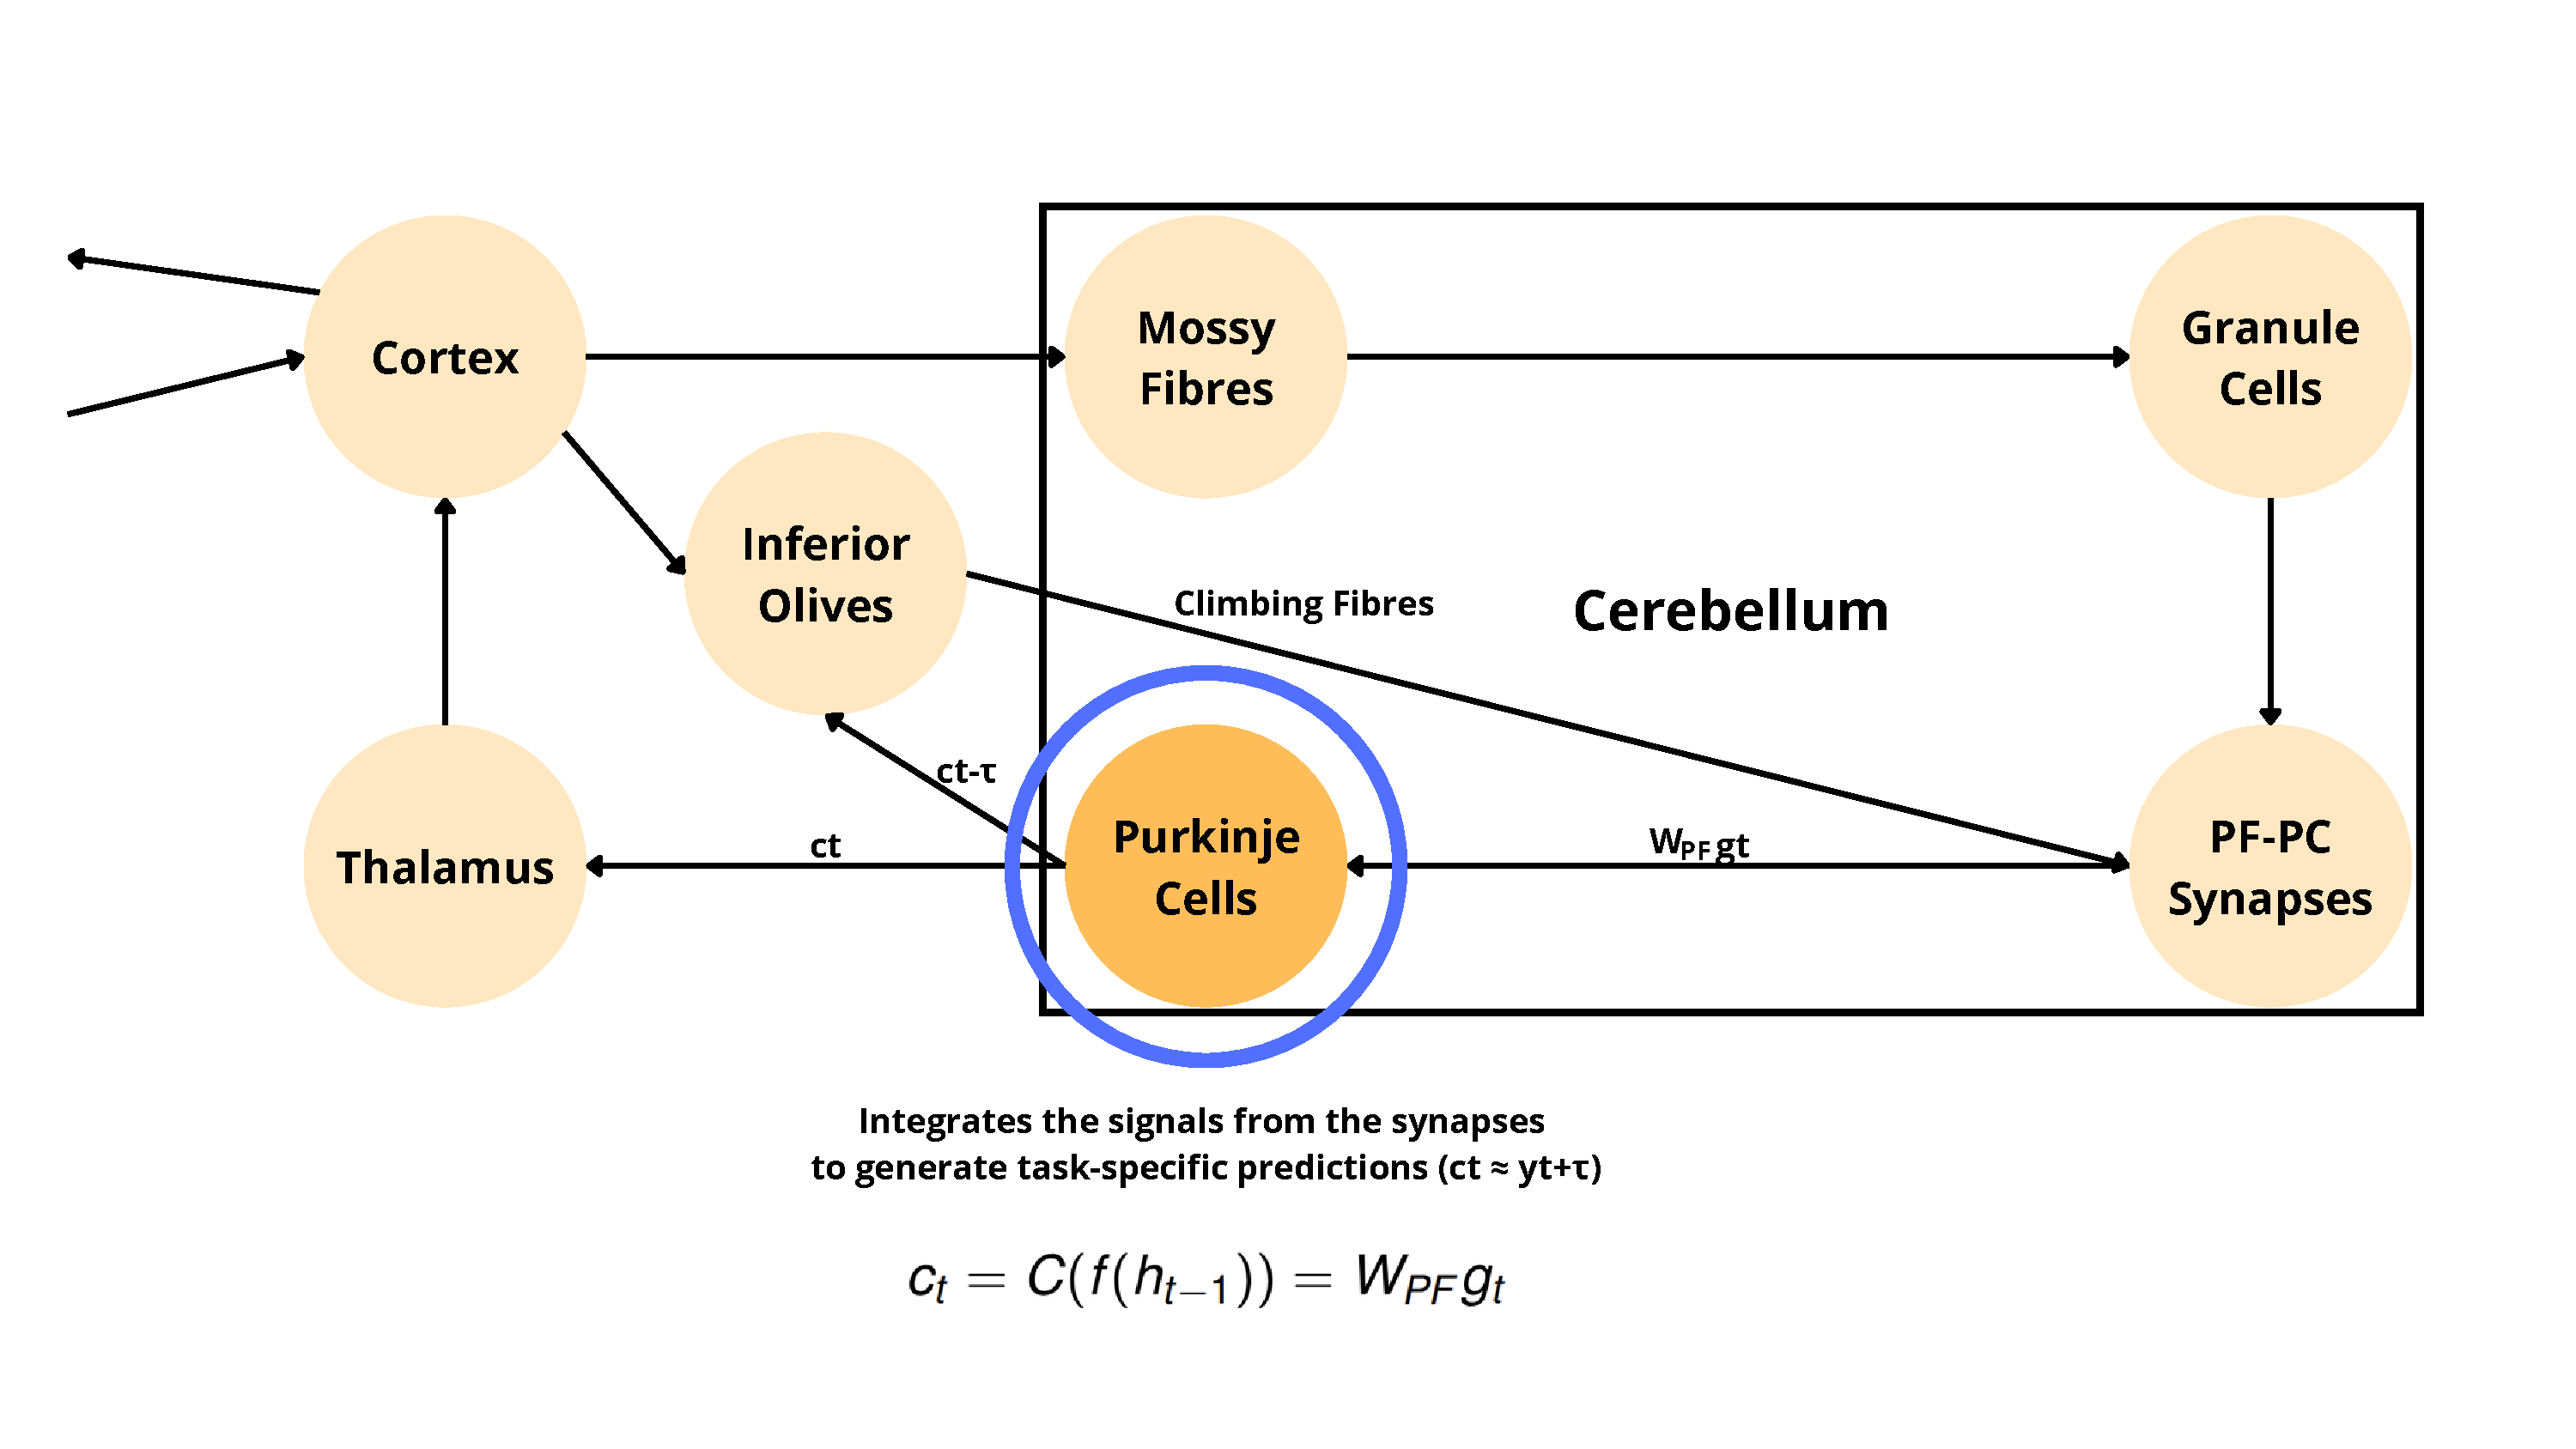
\includegraphics[scale=0.23]{images/cerebellarLoopSchematic/Schema6.pdf}}
    \only<7>{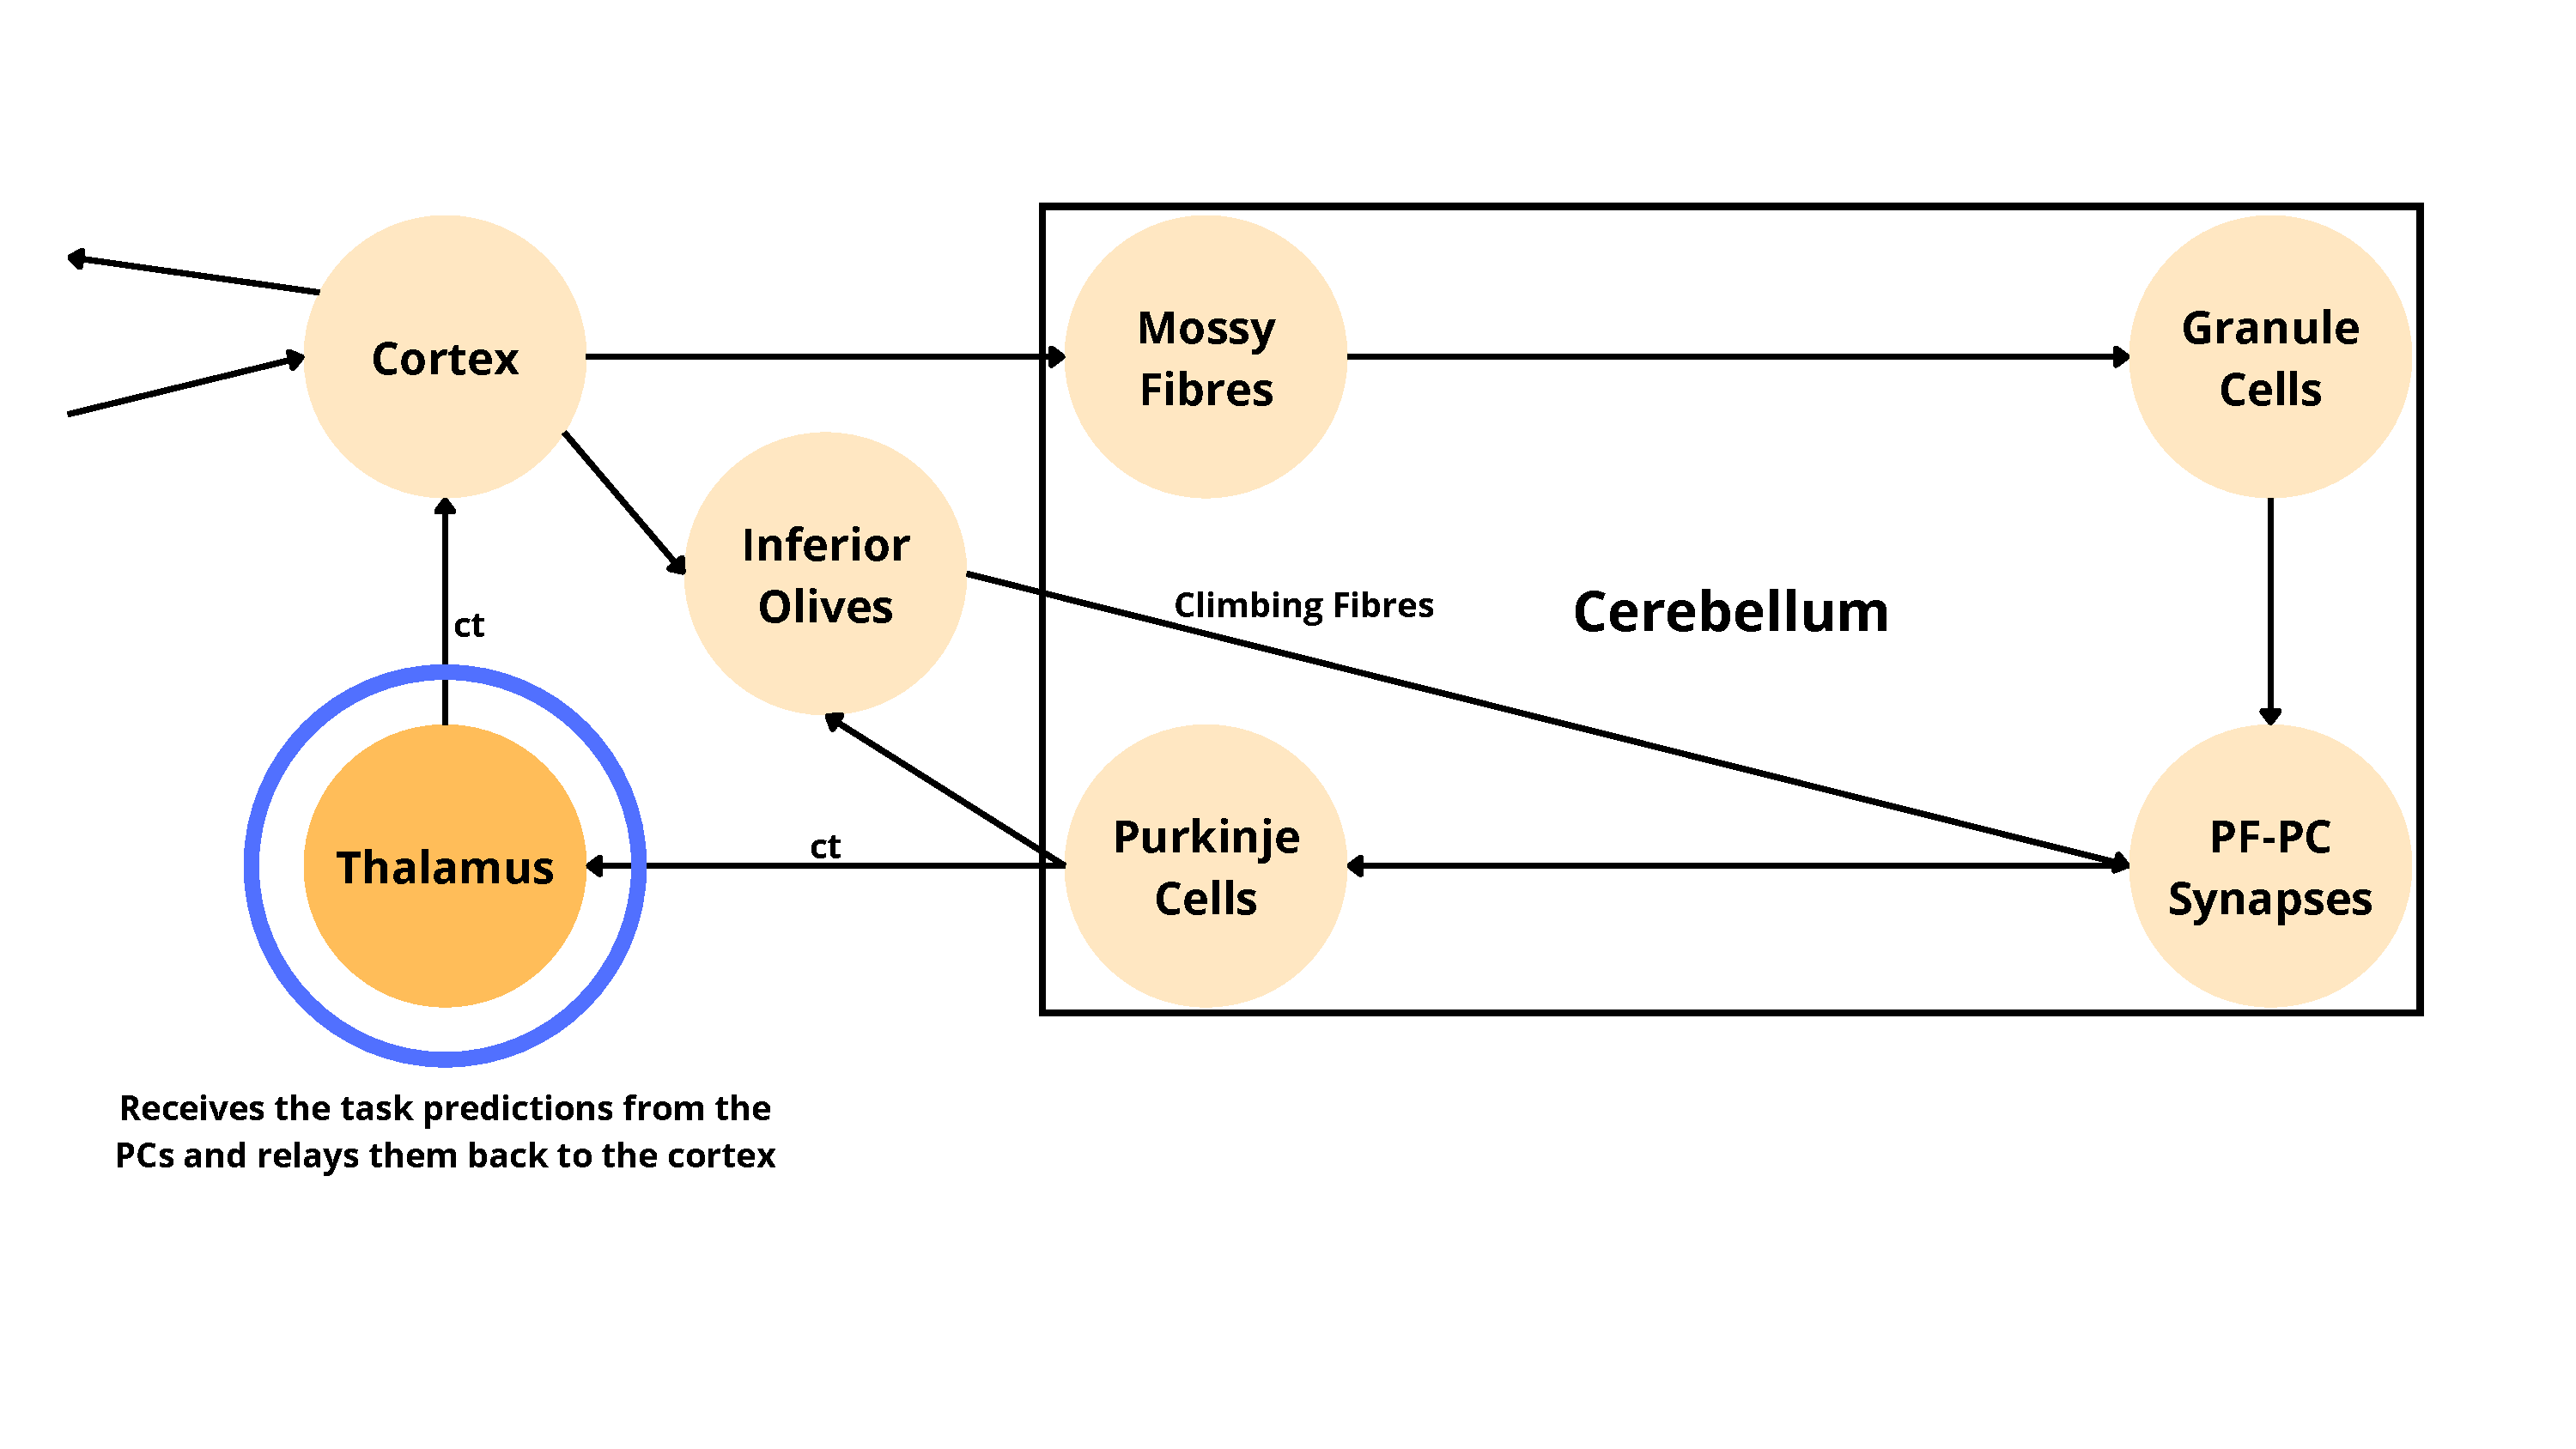
\includegraphics[scale=0.23]{images/cerebellarLoopSchematic/Schema7.pdf}}
    \only<8>{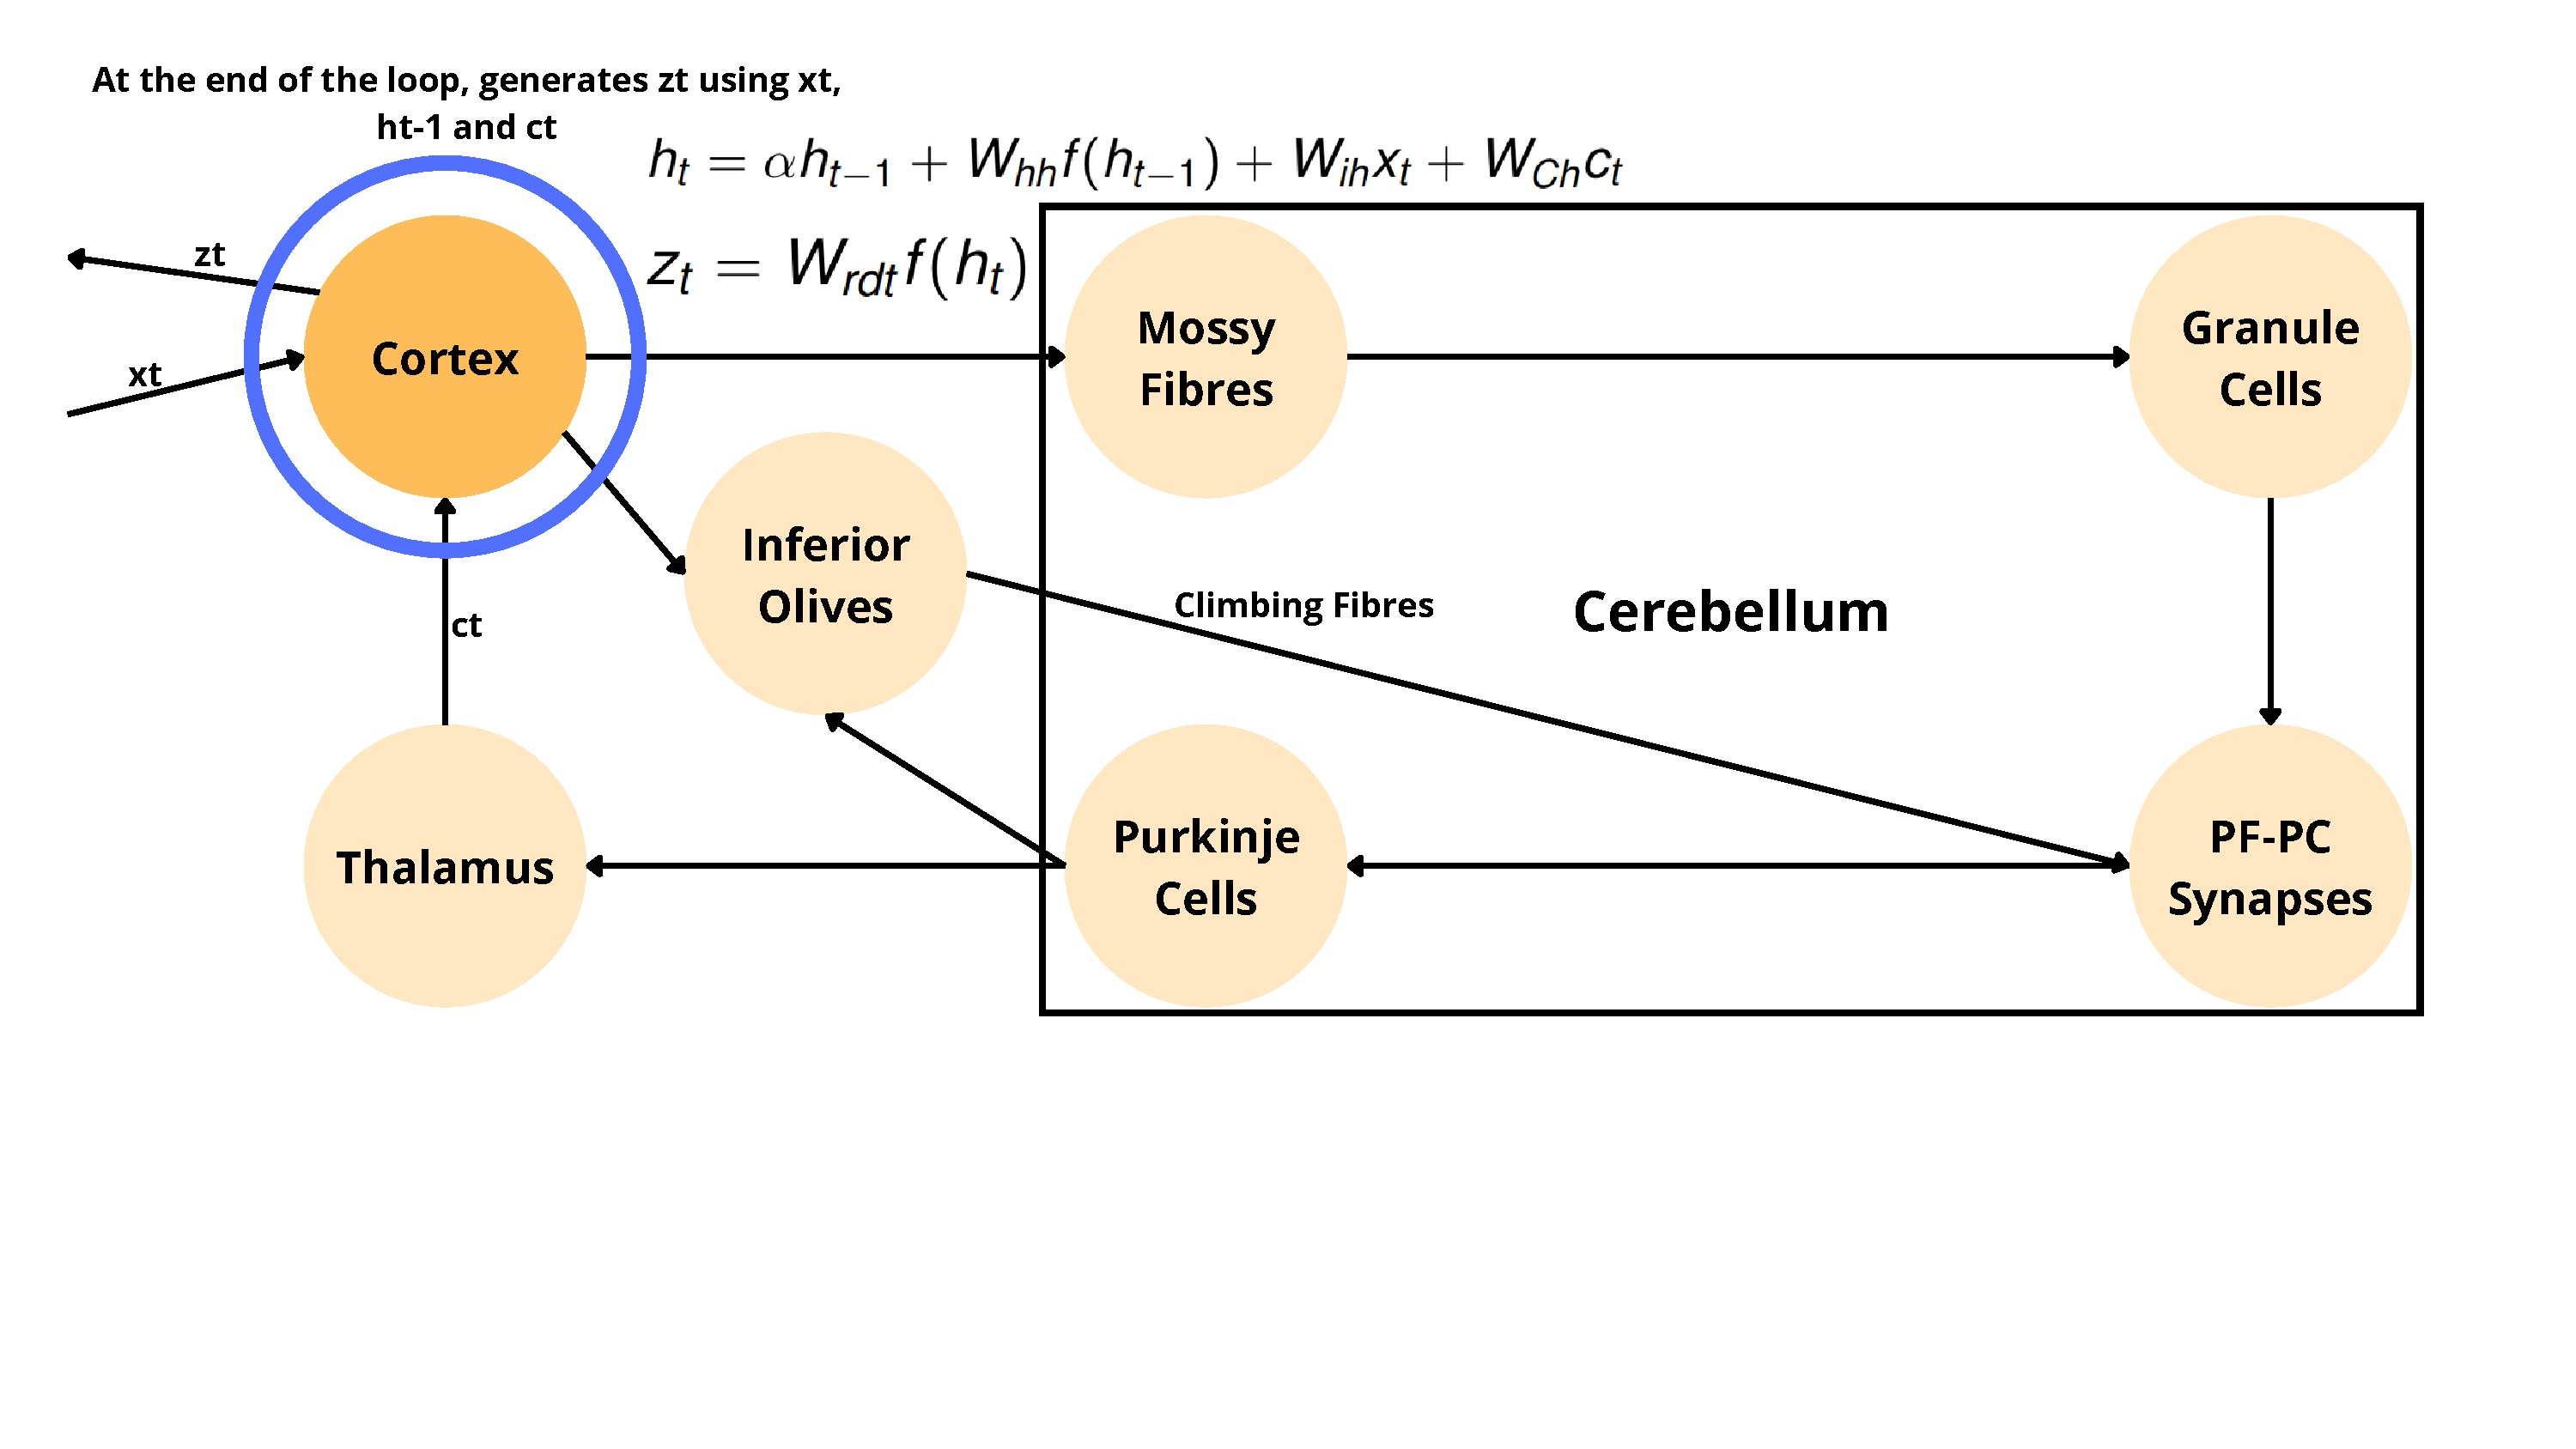
\includegraphics[scale=0.23]{images/cerebellarLoopSchematic/Schema8.pdf}}

\end{frame}

    % x_t: External stimulus.
    % α: Cortical internal memory (leak factor). 
    % W_hh​: Recurrent cortical weights.
    % W_ih​: Stimulus-to-RNN (input) weights.
    % W_Ch​: Cerebellar-to-RNN (feedback) weights.
    % W_PF​: Parallel fiber weights.
    % W_MF​: Mossy fiber weights.
    % z_t​: Final behavioral output (readout).


    % h_t​: Current cortical RNN state.
    % f^C: Cerebellar activation function (ReLU in this case).
    % c_t​: Task prediction generated by the cerebellum. Helps mitigate the "leakiness" of the cortical RNN, driving it towards task-relevant states.
    % f: Cortical activation function (tanh in this case).
    % C: feedforward computation.
    % τ: cerebellar prediction time-window (≈ 150ms (or 3 time steps) for line drawing, ≈ 600ms for evidence accumulation & delayed association tasks)

    % f^C -> ReLU
    % f -> tanh

    \begin{frame}
      \frametitle{Model Training Error Functions}
      \hspace{0.3cm} Two types of error functions are used:
      \vspace{0.5cm}
      \begin{itemize}
        \item \textbf{Task Error:}
          \begin{equation} E_t = \varepsilon(z_t, y_t) \end{equation}
        % where $y_t$ denotes the desired task outcome at time $t$ and $\varepsilon$ is the task error function (MSE for regression, Cross-Entropy loss for classification)
      
      \vspace{0.3cm}

        \item \textbf{Cerebellar Error:}
          \begin{equation} E_t^c = \varepsilon(c_{t-\tau}, y_t) \end{equation}
        % where $\tau$ is the cerebellar learning time window (delay).

      \end{itemize}
    \end{frame}

    \begin{frame}
      \frametitle{Cerebellar Feedback Model}
      \hspace{0.3cm} Three types of cerebellar feedback models are considered: \\
      \vspace{0.5cm}
      \begin{itemize}
        \item \textbf{Fixed RNN:} $W_{hh}$, $W_{ih}$, $W_{MF}$ and $W_{Ch}$ are fixed, while $W_{rdt}$ and $W_{PF}$ are trained.
        \vspace{0.3cm}
        % The internal connectivity of the cortical RNN is fixed and random, and only the input weights are trained. 
        \item \textbf{Input Plastic:} $W_{hh}$ and $W_{MF}$ are fixed, while $W_{ih}$, $W_{rdt}$, $W_{PF}$ and $W_{Ch}$ are trained.
        \vspace{0.3cm}
        % Plasticity is strictly limited to its input synapses 
        \item \textbf{Fully Plastic:} All weights are trained.
      \end{itemize}
    \end{frame}

  \section{Policy-Gradient RL Approach}
    \begin{frame}
      \frametitle{Policy-Gradient RL Approach}
      % The second paper proposes a policy-gradient reinforcement learning approach to model practice-based motor skill learning.
      \begin{figure}
        \centering
        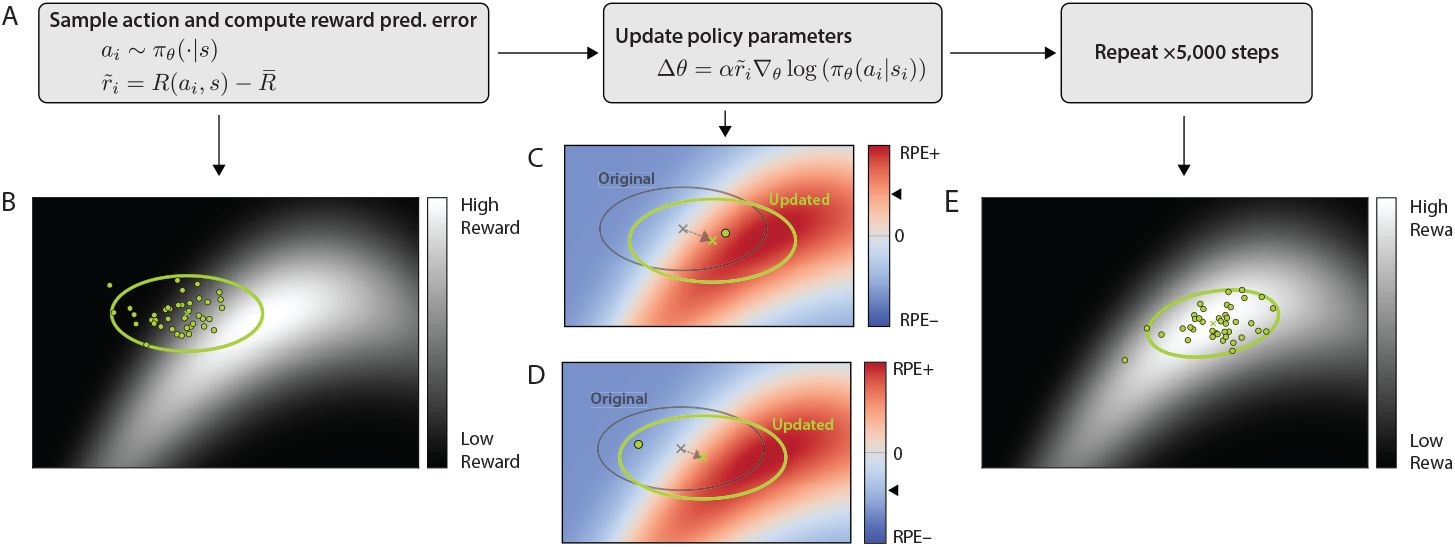
\includegraphics[scale=0.2]{images/policyGradient.jpg}
        \caption{Illustration of policy-gradient RL}
      \end{figure}
    \end{frame}

    % A) Outline of policy gradient algorithm. 
    % B) Reward landscape for a task with 2-dimensional action space, and actions generated according to an initial policy, in this case a 2-dimensional Gaussian. 
      % The green ellipse indicates the covariance of the Gaussian policy (90% confidence interval), while dots represent individual samples. 
    % C) Illustration of policy update for a positive reward prediction error. In this trial, the randomly selected action leads to a beKer-than-average reward (positive reward prediction error). 
      % Consequently, the mean is updated towards the sampled action. 
    % D) Policy update for a negative reward prediction error. Here, the randomly selected action results in a worse-than-average reward (negative reward prediction error). 
      % Consequently, the mean is updated away from the sampled action. 
    % E) After a few thousand samples, the policy converges on the region of greatest reward.

    % Mencionar que vários papers recentes mostram que o cerebelo tem sinais "de RL"

    \begin{frame}
      \frametitle{Model Computational Representation}
      \begin{itemize}
        \item The model represented is of trial-by-trial skill learning:
        \begin{equation}
          \theta_{i+1} = \theta_i + \alpha (r(s_i, a_i) - \bar{r_i}) \frac{\partial}{\partial \theta} \log \pi(a_i|s_i).
        \end{equation}
        \item The average reward $\bar{r_i}$ is also computed on a trial-by-trial basis, according to
        \begin{equation}
          \bar{r}_{i+1} = (1 - \beta) \bar{r_i} + \beta r(s_i, a_i).
        \end{equation}
        \item The policy $\pi(a_i|s_i)$ is assumed to be a Gaussian distribution, with mean $\mu$ and a covariance matrix $\Sigma$:
        \begin{equation}
          \pi(a|s) = \frac{1}{(2\pi)^{\frac{N}{2}} |\Sigma|^{\frac{1}{2}}} e^{-\frac{1}{2}(\mu - a)^T \Sigma^{-1} (\mu - a)}.
        \end{equation}
        where N is the dimensionality of the action space.
      \end{itemize}
    \end{frame}

  \section{Evaluation}
    \begin{frame}
      \frametitle{Evaluation}
      % The implementation will first be evaluated on standard reaching tasks simulated in MuJoCo, such as the Center-Out (CO) and Random Target (RT) tasks, to assess learning performance.
      \begin{figure}
        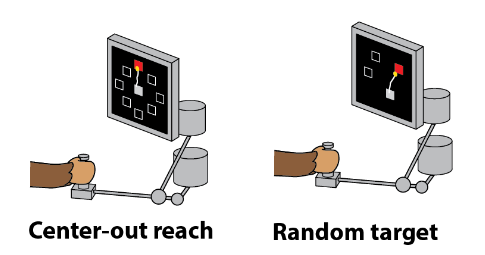
\includegraphics[scale=0.5]{images/CO_RT_Tasks.png} 
      \end{figure}
    \end{frame}

  \section{Environment}
    \begin{frame}
      \frametitle{Environment}
      % The MuJoCo model used for the evaluation is a simplified 2D planar arm with two joints and two degrees of freedom, which allows for efficient simulation and analysis of reaching tasks.
      \begin{figure}
        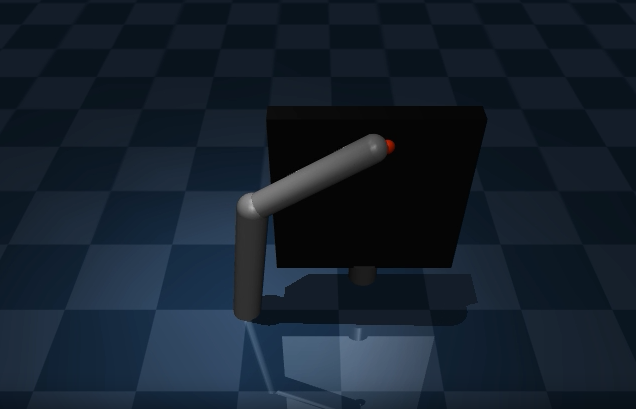
\includegraphics[scale=0.4]{images/mujocoSimpleModel.png}
      \end{figure}
    \end{frame}

  \section{Conclusion}
    \begin{frame}
      \frametitle{Conclusion}
      \hspace{0.3cm} After evaluating both of the paper's approaches, the end goal is to combine the SL and RL frameworks to create a hybrid architecture:
      \begin{figure}
        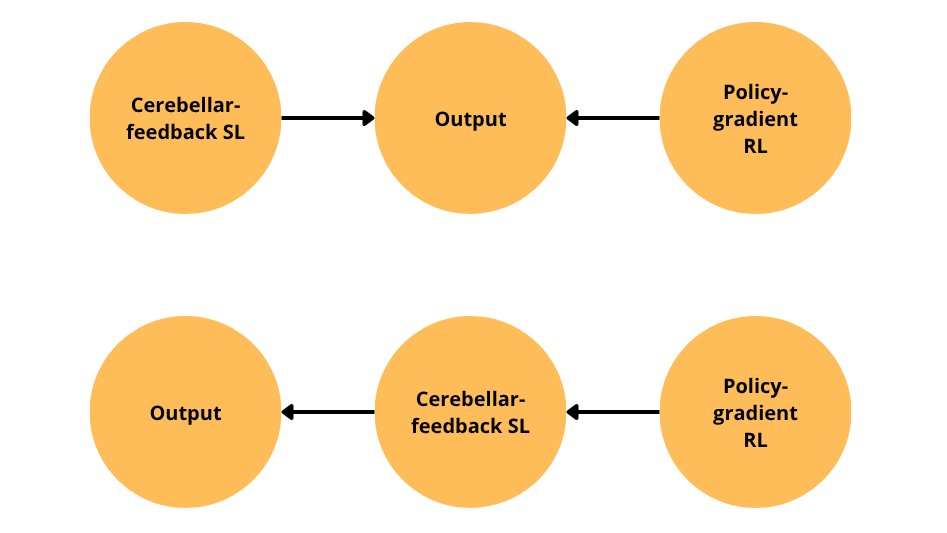
\includegraphics[scale=0.3]{images/hybridModel.png}
      \end{figure}
    \end{frame}
    %  The implementation will first be evaluated on standard reaching tasks simulated in MuJoCo, such as the Center-Out (CO) and Random Target (RT) tasks, to assess learning performance and compare the proposed architecture against conventional recurrent neural network baselines. The ultimate goal is to explore whether cerebellar-inspired feedback mechanisms can improve learning efficiency, stability, and generalization in learning tasks while providing insights into computational principles underlying motor learning in biological systems.
  
\end{document}